\documentclass[twocolumn]{aastex631}

% Packages
\usepackage{microtype}  % ALWAYS!
\usepackage{amsmath}
\usepackage{amsfonts}
\usepackage{amssymb}
\usepackage{multirow}
\usepackage{tikz}
\usepackage{xcolor}
\usepackage{soul}

\definecolor{pink}{RGB}{232,132,161}
\definecolor{yellow}{RGB}{255,213,0}

\newcommand{\kc}[1]{\textcolor{yellow}{\textbf{kc: #1}} }
\newcommand\shadetext[2][]{%
  \setbox0=\hbox{{\special{pdf:literal 7 Tr }#2}}%
  \tikz[baseline=0]\path [#1] \pgfextra{\rlap{\copy0}} (0,-\dp0) rectangle (\wd0,\ht0);% 
  }
\newcommand{\gb}[1]{\shadetext[left color=blue, right color=red, middle color=lime, shading angle=45]{\textbf{g: #1}} }
% \newcommand{\ecite}[1]{\textcolor{pink}{\textbf{: #1}} }
% \newcommand{\e}[1]{\textcolor{yellow}{\textbf{: #1}} }

\newcommand{\remove}[1]{\textcolor{red}{#1}}
\newcommand{\add}[1]{\textcolor{green}{#1}}

\newcommand{\mlg}{\ensuremath{M_{\rm LG}}}
\newcommand{\mmto}{\ensuremath{M_{\rm M31}}}
\newcommand{\mmw}{\ensuremath{M_{\rm MW}}}
\newcommand{\vtan}{\ensuremath{v_\textrm{tan}}}
\newcommand{\vrad}{\ensuremath{v_\textrm{rad}}}
\newcommand{\ms}[1]{\ensuremath{M_{*{#1}}}}
\newcommand{\reflabel}[1]{\ensuremath{^{\mbox{\scriptsize{#1}}}}}
\newcommand{\scsep}{\ensuremath{\rm r_{sep}/r_{vir}}}
\newcommand{\scvel}{\ensuremath{\rm v_{rel}/v_{vir}}}

\newcommand{\paircat}{\textit{Full Pair Catalog}}
\newcommand{\Rvir}{\ensuremath{\rm R_{vir}}}
\newcommand{\Rphys}{\ensuremath{\rm R_{phys}}}
\newcommand{\Rsc}{\ensuremath{\rm R_{sc}}}
\newcommand{\rsep}{\ensuremath{\rm r_{sep}}}

% Style tweaks
% \renewcommand{\twocolumngrid}{\onecolumngrid}
% \setlength{\parindent}{1.1\baselineskip}
% \sloppy\sloppypar\raggedbottom\frenchspacing

%%%%%%%%%%%%%%%%%%%%%%%%%%%%%%%%%%%%%%%%%%%%%%%%%%%%%%%%%%%%%%%%%%%%%%%%%%%%%%%%
\shorttitle{Merger Timescales in TNG100}
\shortauthors{Chamberlain et al.}

%%%%%%%%%%%%%%%%%%%%%%%%%%%%%%%%%%%%%%%%%%%%%%%%%%%%%%%%%%%%%%%%%%%%%%%%%%%%%%%%
\graphicspath{{./}{../plots/}}
% Missions
\newcommand{\project}[1]{\textsl{#1}}

% Packages / projects / programming
\newcommand{\package}[1]{\textsl{#1}}
\newcommand{\acronym}[1]{{\small{#1}}}
\newcommand{\github}{\package{GitHub}}
\newcommand{\python}{\package{Python}}
\newcommand{\astropy}{\package{Astropy}}

% Stats / probability
\newcommand{\given}{\,|\,}
\newcommand{\norm}{\mathcal{N}}
\newcommand{\pdf}{\textsl{pdf}}

% Maths
\newcommand{\dd}{\mathrm{d}}
\newcommand{\transpose}[1]{{#1}^{\mathsf{T}}}
\newcommand{\inverse}[1]{{#1}^{-1}}
\newcommand{\argmin}{\operatornamewithlimits{argmin}}
\newcommand{\mean}[1]{\left< #1 \right>}

% Non-scalar variables
\renewcommand{\vec}[1]{\ensuremath{\bs{#1}}}
\newcommand{\mat}[1]{\ensuremath{\mathbf{#1}}}

% Unit shortcuts
\newcommand{\Msun}{\ensuremath{\mathrm{M}_\odot}}
\newcommand{\Mjup}{\ensuremath{\mathrm{M}_{\mathrm{J}}}}
\newcommand{\kms}{\ensuremath{\mathrm{km}~\mathrm{s}^{-1}}}
\newcommand{\pc}{\ensuremath{\mathrm{pc}}}
\newcommand{\kpc}{\ensuremath{\mathrm{\,kpc}}}
\newcommand{\Mpc}{\ensuremath{\mathrm{Mpc}}}
\newcommand{\kmskpc}{\ensuremath{\mathrm{km}~\mathrm{s}^{-1}~\mathrm{kpc}^{-1}}}
\newcommand{\dayd}{\ensuremath{\mathrm{d}}}
\newcommand{\yr}{\ensuremath{\mathrm{yr}}}
\newcommand{\Myr}{\ensuremath{\mathrm{Myr}}}
\newcommand{\Gyr}{\ensuremath{\mathrm{\,Gyr}}}
\newcommand{\Kel}{\ensuremath{\mathrm{K}}}
\newcommand{\masyr}{\ensuremath{\mathrm{mas}~\mathrm{yr}^{-1}}}
\newcommand{\muasyr}{\ensuremath{\mu\mathrm{as}~\mathrm{yr}^{-1}}}

% Misc.
\newcommand{\bs}[1]{\boldsymbol{#1}}

% Astronomy
\newcommand{\DM}{{\rm DM}}
\newcommand{\feh}{\ensuremath{{[{\rm Fe}/{\rm H}]}}}
\newcommand{\df}{\acronym{DF}}

% TO DO
\newcommand{\todo}[1]{{\color{red} TODO: #1}}
\newcommand{\apw}[1]{{\color{blue} APW says: #1}}

% Projects
\newcommand{\gaia}{\textsl{Gaia}}
\newcommand{\gaiadr}{\textsl{Gaia}~\acronym{EDR3}}
\newcommand{\hst}{\textsl{HST}}

% Paper specific
\newcommand{\paircat}{\textit{Full Pair Catalog}}

\newcommand{\lcdm}{\ensuremath{\Lambda \rm CDM}} 
\newcommand{\sublink}{\textsc{sublink}} 
\newcommand{\subfind}{\textsc{subfind}} 

% masses - halo
\newcommand{\Mpeak}{\ensuremath{M_{\mathrm{peak}}}}
\newcommand{\Mhalo}{\ensuremath{M_{\mathrm{h}}}}
\newcommand{\MG}{\ensuremath{\rm M_{\mathrm{G}}}}
\newcommand{\mlg}{\ensuremath{M_{\rm LG}}}

% masses - stellar
\newcommand{\Ms}{\ensuremath{\rm M_{{*}}}}
\newcommand{\msam}{\ensuremath{M_{*,\mathrm{am}}}}
\newcommand{\mssim}{\ensuremath{M_{*,\mathrm{sim}}}}
\newcommand{\ms}[1]{\ensuremath{M_{*{#1}}}}

\newcommand{\vtan}{\ensuremath{v_\textrm{tan}}}
\newcommand{\vrad}{\ensuremath{v_\textrm{rad}}}
\newcommand{\reflabel}[1]{\ensuremath{^{\mbox{\scriptsize{#1}}}}}

\newcommand{\Rvir}{\ensuremath{\rm R_{vir}}}
\newcommand{\Rphys}{\ensuremath{\rm R_{phys}}}
\newcommand{\Rsc}{\ensuremath{\rm R_{sc}}}
\newcommand{\rsep}{\ensuremath{\rm r_{sep}}}

% Affiliations
\newcommand{\affuofa}{University of Arizona, 933 N. Cherry Ave,
    Tucson, AZ 85721, USA}

\newcommand{\affuofu}{Department of Astronomy, University of Utah, Salt Lake City, UT 84112, USA}

\begin{document}

\title{A Physically Motivated Framework to Compare Merger Timescales\\ of Isolated Low- and High-Mass Galaxies Across Cosmic Time
}

\author[0000-0001-8765-8670]{Katie~Chamberlain}
\affiliation{\affuofa}

\author[0000-0002-9820-1219]{Ekta~Patel}
\thanks{Hubble Fellow}\affiliation{\affuofu}


\author[0000-0003-0715-2173]{Gurtina Besla}
\affiliation{\affuofa}




\author{others}

\begin{abstract}
% Statement
Evolutionary differences between low-mass ($\rm 10^8<M_*<5\times10^9\,\Msun$) and high-mass ($\rm 5\times10^9<M_*<10^{11}\,\Msun$) galaxy pairs have been studied in detail for the last few decades, with studies finding differences in star formation rates, gas fractions, and dark matter halo profiles. 
% Problem 
However, many studies continue to use equivalent separation criteria to select galaxy pairs for pair fraction, merger fraction, and merger rate studies, though it is unclear that such a selection permits an equitable comparison between galaxies of different mass, nor as a function of redshift.   
% Our solution
We use the Illustris TNG100 simulation to quantify the merger timescales of isolated low-mass and high-mass major pairs as a function of cosmic time. 
% What are the timescales? 
We show that separation limits that vary with the mass and redshift of the system, such as scaling by the virial radius of the host halo ($r_{\mathrm{sep}}< 1 R_{\rm vir}$), lead to equivalent merger timescales for low- and high-mass systems at all redshifts. 
Alternatively, static physical separation selections applied equivalently to all galaxy pairs at all redshifts, particularly for the closest pairs ($\rsep<150\kpc$) leads to timescales that differ between low- and high-mass pairs. 
% Why it matters 
Our findings suggest that the comparison of low-mass and high-mass galaxy pair fractions, merger timescales, and merger rates must be done with self-consistent separation criteria that scales as a function of mass and redshift of the system. 
As a result, applying the same merger timescales to different mass systems will lead to a bias that systematically (over/under) predicts low-mass galaxy merger rates. 
\end{abstract}

%%%%%%%%%%%%%%%%%%%%%%%%%%%%%%%%%%%
\section{Introduction} \label{sec:intro}

% $z=1.5$ corresponds to snapshot \#40 in the TNG sim
% Introduce RG15, Lotz, etc.



%%% OUTLINE
\section{Methodology}
%recap last paper and mention which data sample we narrow down to (low mass major pairs only) -- give examples of orbits
We utilize the group catalogs, produced by the \texttt{SUBFIND} algorithm~\citep{Springel2001,Dolag2009}, and the merger tree catalogs, generated by the \texttt{SUBLINK} algorithm~\citep{RG2015}, from the highest resolution run of the IllustrisTNG simulation TNG100-1 (hereafter TNG100) to study the merger timescales of galaxy pairs from $z=0-XX$.

Our sample consists of major low-mass and high-mass pairs that are isolated but physically associated.
From this sample, we will determine the fraction of pairs at each snapshot that merge before $z=0$, and track the orbits of the subhalos of each pair to study their merger timescales.


\subsection{Pair orbit sample}
We begin with a subset of the \paircat{} described in ~\citet{Chamberlain2024}, which consists of a collection of isolated subhalo pairs at each snapshot in TNG100. 
A brief version of the selection routine is described here. 

At each snapshot, low-mass and high-mass pairs are chosen by first selecting the two most massive halos (by stellar mass) from FoF groups with virial mass\footnote{We use \texttt{Group\_M\_TopHat200} from the TNG100 Group Catalogs as the FoF Group virial mass. This mass is defined to be the mass enclosed by a sphere with mean density $\Delta_c *\rho_c$, where $\Delta_c$ is the overdensity constant from~\citet{Brynorman1998} and $\rho_c$ is the critical density of the universe at the time calculated. The corresponding virial radius in TNG100 is given by \texttt{Group\_R\_TopHat200}.} 
\begin{align*}
        \mbox{\textbf{low mass:}}&\,\rm M_{G} = 8\times 10^{10}- 5\times 10^{11}\,\Msun \\ 
        \mbox{\textbf{high mass:}}&\, \rm M_{G}=10^{12}- 6.5\times10^{12}\,\Msun.
\end{align*}
Utilizing the most massive subhalos from the same FoF group ensures that the pairs are isolated from massive nearby systems that may perturb the dynamical state of the pair. 

We require that subhalos that constitute a pair meet a minimum subhalo mass criteria of 
\begin{equation*}
    \mbox{\textbf{minimum subhalo mass:}}\,
    \Mhalo > 1\times10^{9}\Msun.
\end{equation*}
at the snapshot of consideration. 
For each halo in the FoF group that passes the minimum subhalo mass criteria, we utilize the \texttt{SUBLINK} catalogs to trace their mass history~\citep{RG2015}, and find the peak halo mass of each subhalo. 

Stellar masses are then assigned to each subhalo in the FoF group using the Abundance Matching prescription of \citet{Moster2013}. 
The peak halo mass and current snapshot are used to calculate the stellar mass of each subhalo, so that the abundance matching prescription is of the form $\ms{}=f(\Mpeak,z_{\mathrm{snap}})$.

In \citet{Chamberlain2024}, the abundance matching prescription is sampled 1000 times for each subhalo to account for the spread in the abundance matching prescription. 
However, for the purposes of the present study, we only use the stellar masses given by the median of the abundance matching relationship. 
This choice allows us to more thoroughly consider the population under study, and also permits a roughly 1:1 monotonic relationship between stellar mass and peak halo mass, so that taking subsamples of the lowest stellar mass objects will result in a subsample with lower peak halo mass as well. % is this a good enough reason? 
% else, maybe spread of number of pairs is so small, that we expect the noise of the timescale analysis to be dominated by the snapshot spacing anyways? 

Primary halos are defined as the subhalo with the highest stellar mass ($M_{*1}$) in their FoF group, and secondaries are defined as the second most massive subhalo with stellar mass $M_{*2}$. 
Our sample of major pairs then consists of all pairs of primary and secondary halos with 
\begin{align*} 
\mbox{\textbf{low mass primaries:}}&\, 10^{8}< \rm M_{*1} < 5\times10^{9} \Msun \\ 
\mbox{\textbf{high mass primaries:}}&\, 5\times 10^{9}< \rm M_{*1} < 10^{11} \Msun\\
\mbox{\textbf{stellar mass ratio:}}&\,      
    M_{*2}/M_{*1} > 1/4.
\end{align*}
A primary or secondary halo can only be a member of one single pair at a given snapshot, such that a collection of $N$ pairs consists of $N$ unique primaries and $N$ unique secondaries.

% i am removing the 10kpc component of this because I think it'd just be easier to handle those cases in the 
% Finally, we will only consider pairs that have physical separations of $\rsep>10\,\kpc$ at the snapshot of selection. 
% The physical separation cut does not vary with redshift, and is the same for both low-mass and high-mass pairs. 

The base sample used for this analysis then consists of the set of all low-mass and high-mass major pairs from each snapshot of the TNG100 simulation. 


\subsubsection{Mergers}
% Plot \#1: Merger fraction either before or after orbits
% Note that it is very interesting that dwarf pairs in the field have high merger fractions, while the likelihood of merger is very low in more dense environments (add citation).

The primary and secondary subhalos of each pair have a `SubfindID' that is used to identify them in the \texttt{Subfind} catalogs, which contain information about every FoF group and subhalo at each snapshot. 
The \texttt{SUBLINK} catalogs track subhalos from one snapshot to the next, and thus enable us to track subhalos both backwards and forwards in time from any given snapshot. 

We utilize the \texttt{RootDescendantID} and \texttt{DescendantID} fields of the \texttt{SUBLINK} catalogs to determine which pairs from our base sample merge before the end of the simulation (at $z=0$), and to determine when the merger occurs. 
The \texttt{DescendantID} field provides the `SubhaloID'\footnote{Note that the `SubhaloID' is distinct from the `SubfindID', and is unique for every subhalo in the merger trees. 
The \texttt{SUBLINK} catalogs provide the associated `SubfindID' of each subhalo.} of the subhalo's descendent in the next (or one of the following) snapshot, if it has one. 
% By following the \texttt{DescendantID}, you follow a subhalo through all of it's mergers to the `root' of the merger tree.  
The \texttt{RootDescendantID} field provides the SubhaloID of the root subhalo, which is the latest subhalo in the simulation that is a descendent of the subhalo.  

We define the set of merging pairs as the collection of all pairs where the primary and secondary halo have the same \texttt{RootDescendantID}, meaning that the branches of their merger trees have the same `root', or common descendent. 
If a given pair has two distinct \texttt{RootDescendantID} values, the pair is defined as a `non-merger.'

For each merging pair, we define the `merger snapshot' as the snapshot that immediately follows the first snapshot where the primary and secondary have the same \texttt{DescendantID}. 
For example, if the primary and secondary have different \texttt{DescendantIDs} for snapshots 40-45, but have the same \texttt{DescendantID} at snapshot 46, then the merger must take place some time between snapshot 46 and 47. 
We take snapshot 47 to be the merger snapshot. 



\subsubsection{Orbits} 
We calculate orbits for all mergers and non-mergers in our base sample. 
An orbit for a single pair is defined to be the physical separation between the primary and secondary halo as a function of redshift or Lookback Time. 

A given pair from the base sample at snapshot $S_n$, which by definition passes all selection criteria at $S_n$, can be followed backwards and forwards in time using the \texttt{SUBLINK} merger trees.  
We track the positions of both the primary and secondary subhalo at each snapshot and calculate the physical separations after accounting for the periodic boundary conditions of the simulation box.
In cases where the primary or secondary does not have a defined position at a given snapshot, we set the separation at that snapshot to NaN.\footnote{If a subhalo is very small, or is passing through a more massive subhalo, and is unable to reach the density contrast required to be identified as an independent structure by the Subfind algorithm, it will not have a defined position in the Sublink catalogs. The sublink algorithm allows for subhalos to skip a single snapshot, and identifies the `skipped descendent' in the $S_{n+2}$ snapshot, so that the orbit can be computed contiguously for a pair on . See Sec.~3 in ~\citet{RG2015} for more details.}

In addition to the physical separation, we also calculate the scaled separation of a pair at each snapshot. We use the definition of scaled separation from~\cite{Chamberlain2024}, given as
\begin{equation}
    \rm \Rsc = \frac{\rsep}{\Rvir}
\end{equation}
where $\rsep$ is the physical separation in $\kpc$, and $\Rvir$ is the virial radius of the primary's FoF group, which reasonably approximates the virial radius of a halo with a virial mass equal to the combined subhalo mass of the primary and secondary.
The scaled radius $\Rsc$ is by construction a function of mass and redshift, which will account for the mass difference between low-mass and high-mass pairs, or for halo growth over time. 

We collect the following data for each pair at each snapshot where the primary and secondary are both defined: the virial mass of the primary's FoF group \texttt{Group\_M\_TopHat200}, the virial radius of the primary's FoF group \texttt{Group\_R\_TopHat200}, the physical separation (in $\kpc$), and the scaled separation (dimensionless).

\subsubsection{"First Infall"}
The orbit of a pair may be technically defined at very early times, well before the primary and secondary are physically associated. 
However, we wish to constrain our orbital analysis to only physically associated pairs, and thus will not consider the orbit of a subhalo pair before they are a part of the same FoF group. Specifically, we will consider only the "Post-Infall" part of each pair's orbit. 

We define the snapshot of "First Infall" as the first snapshot where the primary and secondary have the same parent FoF halo, and "Post-Infall" as the set of snapshots including the snapshot of "First Infall" and all snapshots thereafter. 
The post-infall orbit definition is slightly more robust for considering the full interaction timescales of merging pairs than only considering the orbit when the FoF group of the primary and secondary are the same. 
This is because there are cases of pair interactions where the secondary will enter the FoF group of the primary, have a pericentric passage, then leave the FoF group for a few gigayears before re-entering the primary FoF group and eventually merging with the primary. 

An example of the orbit of a merging pair where a "common group" criteria may differ from a "post-infall" can be seen in Figure~\ref{fig:example-orbits}, which shows the variety of orbits that can be found in the TNG100 simulation for pairs that were originally selected at $z=1.5$. 
The top panel shows the orbits of 5 pairs that merge, where solid lines show the parts of the orbit that occur while the primary and secondary share a common FoF group, and dashed lines show the parts of the merger where the FoF group of the secondary is different than that of the primary. 
The "post-infall" part of the orbit occurs after the first snapshot where the solid lines begins.
Pairs chosen at $z=1.5$ on average merge at $z=XX$/within XX Gyrs, though the spread of merger timescales is large, leading to a single redshift-selected sample having merger timescales between $\sim1-10\Gyr$.


The middle panel shows the orbits for 3 pairs that are classified as non-mergers, since they do not merge before $z=0$, but which appear likely to merge within a couple Gyr past the end of the simulation, and are thus "Potential Future Mergers". 
These orbits can have a variety of orbital periods, and the number of pericentric passages can vary significantly. 
The two lighter blue orbits are very long period orbits with 1-2 pericenter passages in the past 10Gyr, while the darker blue orbit has a much shorter period with many close encounters throughout, and 3 close passages in just the past 2 Gyr.
The bottom panel shows the orbits of "Fly-by" interactions (non-mergers) that are unlikely to merge in the near future, if ever.  
Note that we do not split our non-merger category into fly-bys and potential future mergers for any of our following analyses, and such distinctions were made only for the purposes of showing the diversity of orbits that pairs selected at the same snapshot may follow.

\begin{figure}[htb]
    \begin{center}
    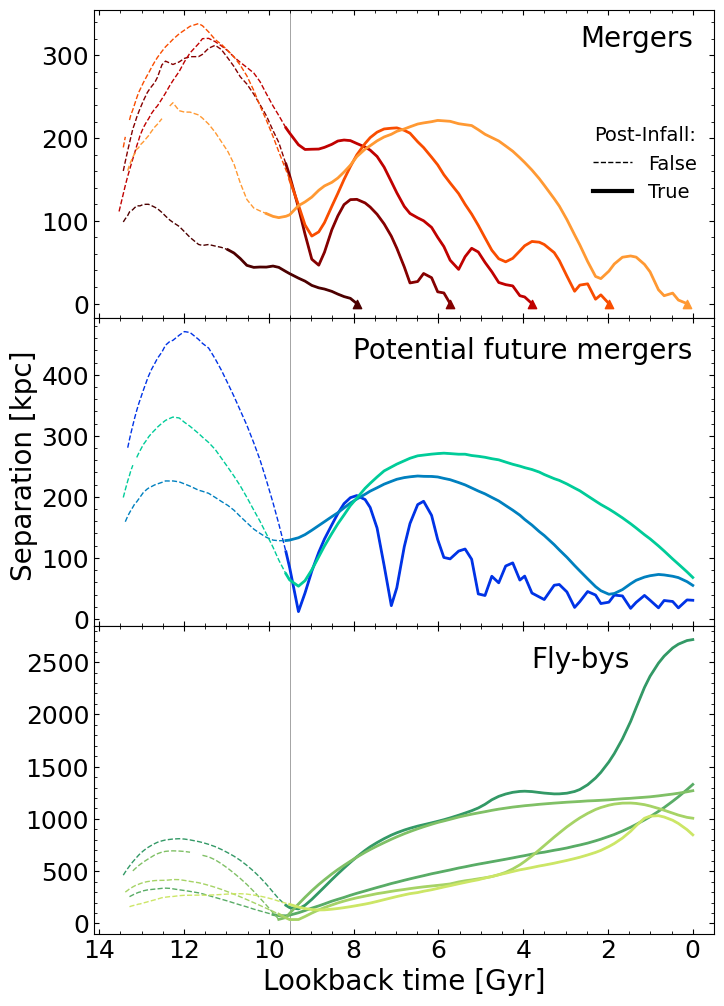
\includegraphics[width=\columnwidth, trim={0.4cm 1.75cm 1cm 3.5cm}, clip]{plots/bet-on-it/5_exampleorbits.png}
    \caption{Selection of example orbits of low-mass major pairs selected at $z=1.5$, showing the separation between the primary and secondary halo of the pair as a function of Lookback Time. The vertical grey line marks $z=1.5$ at a Lookback Time of $9.5\,\Gyr$.
    Solid lines represent the parts of the orbit where the primary and secondary halo have the same FoF group, while the dashed lines show where they are not within the same FoF group. 
    (Top) Orbits of pairs that merge before $z=0$. Pairs chosen at $z=1.5$ on average merge at \kc{$z=XX$/within XX Gyrs}.
    (Middle) Orbits of pairs that did not merge before $z=0$ (non-mergers), but are likely to merge if the simulation continued. 
    (Bottom) Orbits of pairs that did not merge before $z=0$ (non-mergers) and are unlikely to do so in the future $\sim2\Gyr$ (past the end of the simulation). 
    }
    \label{fig:example-orbits}
    \end{center}
\end{figure}


\subsubsection{Uniqueness of pairs}
Since our entire pair sample consists of pairs chosen at separate snapshots, and since a single pair could pass our selection criteria at many snapshots, we keep only a single orbital instance of each pair. 

To distinguish pairs from one snapshot to another, each pair is assigned a pairkey while constructing their orbit, which is created by combining the primary's and secondary's earliest SubhaloID from the Sublink catalogs, which will be unique for each pair of halos. 
After each pair is assigned a unique pairkey, we save the orbit as a function of time only once for a pair that otherwise would have been double/multi-counted in our orbit catalog.

For $n_k$ the number of pairs selected at snapshot $S_k$ via the selection criteria/from the base sample, the total number of pairs is given by
\begin{equation*}
    \sum_{k=0}^{99}\, n_k
\end{equation*}
The total number of low-mass pairs is 71,429, and the total number of high-mass pairs is 20,824.
After selecting only unique pairs, there remain 22,213 unique low-mass pairs, and 3,029 unique high-mass pairs.

Note that a single subhalo may be a member of many different pairs, but will only have one unique orbit per unique pair.
For example, the primary of a low-mass pair selected at $z=3$ that merges before $z=2$ may be selected via our selection criteria again at $z=1$ with a new secondary companion. 
In this case, both orbits (of the original low-mass pair and the new pair which includes the remnant subhalo from the previous merger) are kept, since having the primary occur twice in the catalog does not mean that the orbit is being double counted. ugh. 


Maybe need to define the "unique pair sample" and the "snapshot selected sample" to explain the plots? I think all plots EXCEPT the merger fraction are with unique pair sample.... DO I need to change that plot? 
% \subsection{Calculating the Number of Unique Pairs}

% \subsection{Calculating the Merger Fraction}

% \subsection{Calculating the Time Until Merger}


\section{Pair Sample Properties}
\subsection{Number of Unique Pairs}
We calculate the number of unique pairs at a given snapshot by selecting all unique pairs at that snapshot that have already experienced first infall, and then sum the number of pairs that have yet to merge.
Thus, the total number of unique pairs at $z=2$ includes pairs that were added to the catalog at \textit{any} snapshot, provided they achieved first infall at $z\geq2$ and have a merger redshift $z<2$. 
A single pair (for example, a pair that was first selected in the snapshot-selected catalogs at $z=1$) may meet the conditions of being a "post-infall + pre-merger" pair for $z=0-3$, and will thus contribute to the number of unique pairs at all redshifts from $z=0-3$. 

In Fig.~\ref{fig:num-pairs}, we show the number of low-mass and high-mass unique pairs as a function of redshift from $z=0-6$. 
Unique low-mass pairs (green solid line) are most numerous between $z=1.25-2$, while unique high-mass pairs (pink solid line) are most numerous between $2=0-1$.
The dashed lines show the number of unique pairs that merge prior to $z=0$ for each sample. 
The number of pairs that merge decreases to 0 at $z=0$ since pairs selected at $z=0$ by definition have not merged, and thus will not have the chance to, and low redshift selected pairs will on average have merger timescales longer than the remaining time to the end of the simulation. 

The light green and light pink shaded regions show the number of pairs selected at each snapshot individually, so pairs at $z=1$ that do not pass the snapshot-selection criteria at $z=2$ are not included in the number of pairs at $z=2$, but may still be counted at all snapshots where the selection criteria are met. 
These lines are identical to the pair count lines for low-mass and high-mass pairs from Fig.~1 in~\cite{Chamberlain2024}.

\begin{figure}[htb]
    \begin{center}
    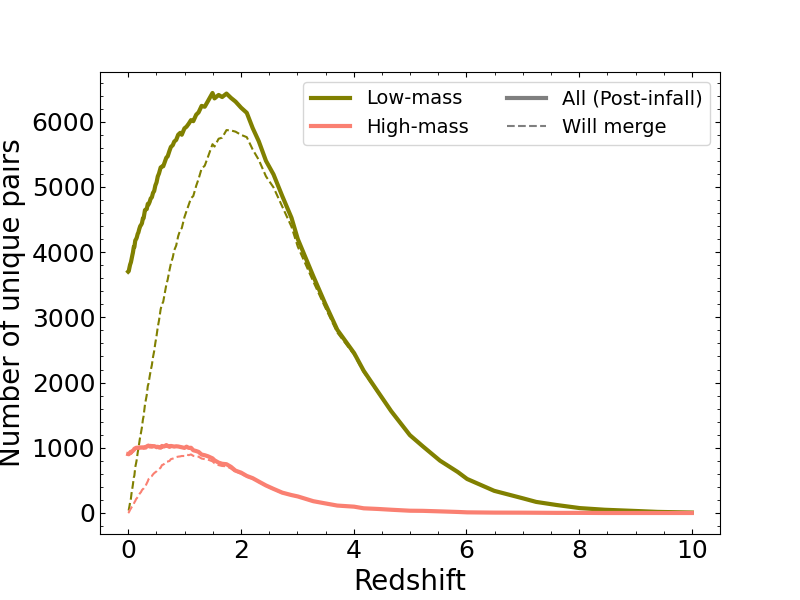
\includegraphics[width=\columnwidth]{plots/bet-on-it/3_number_pairs.png}
    \caption{\kc{change redshift range to 0-6}, add \# pairs from pears, change dash to dots}
    \label{fig:num-pairs}
    \end{center}
\end{figure}



\subsection{Merger Fraction}

\begin{figure}[htb]
    \begin{center}
    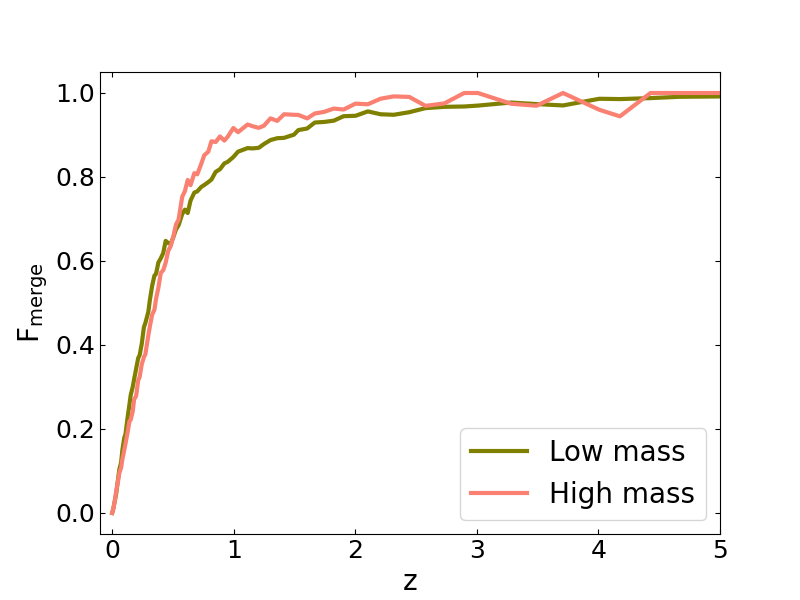
\includegraphics[width=\columnwidth]{plots/bet-on-it/1_fmerge_comp.png}
    \caption{The fraction of pairs that merge before z=0 as a function of the redshift where they were selected via the selection criteria for the \paircat{} from \citet{Chamberlain2024}. At $z>1$, the fraction of selected pairs that merge before $z=0$ is upwards of 80\% for both low mass and high mass isolated pairs. The sharp decline to $F_{\rm merge}$ at $z=0$ is a non-physical feature of the simulation ending at $z=0$, thus unable to follow the pairs after the simulation ends to see what fraction of pairs may have merged.}
    \label{fig:fmerge}
    \end{center}
\end{figure}


% ###########################################################################################
% Results II 
% ###########################################################################################

\section{Results - The Mass and Redshift Dependence of Merger Timescales}
% The point of this subsection: to show that using the same "observability times" for pairs selected in the same physical separation bins wouldn't work, and that the selection criteria for close pairs should either be scaled with mass and redshift. 
\subsection{"time til merger" for selected snapshots for LvH.}
Maybe also (distribution plot 2D hist? as function of selected separation)
\subsection{Cumulative distributions}
\subsubsection{Physical}
\subsubsection{Scaled}

% \begin{figure*}[htb]
%     \centering
%     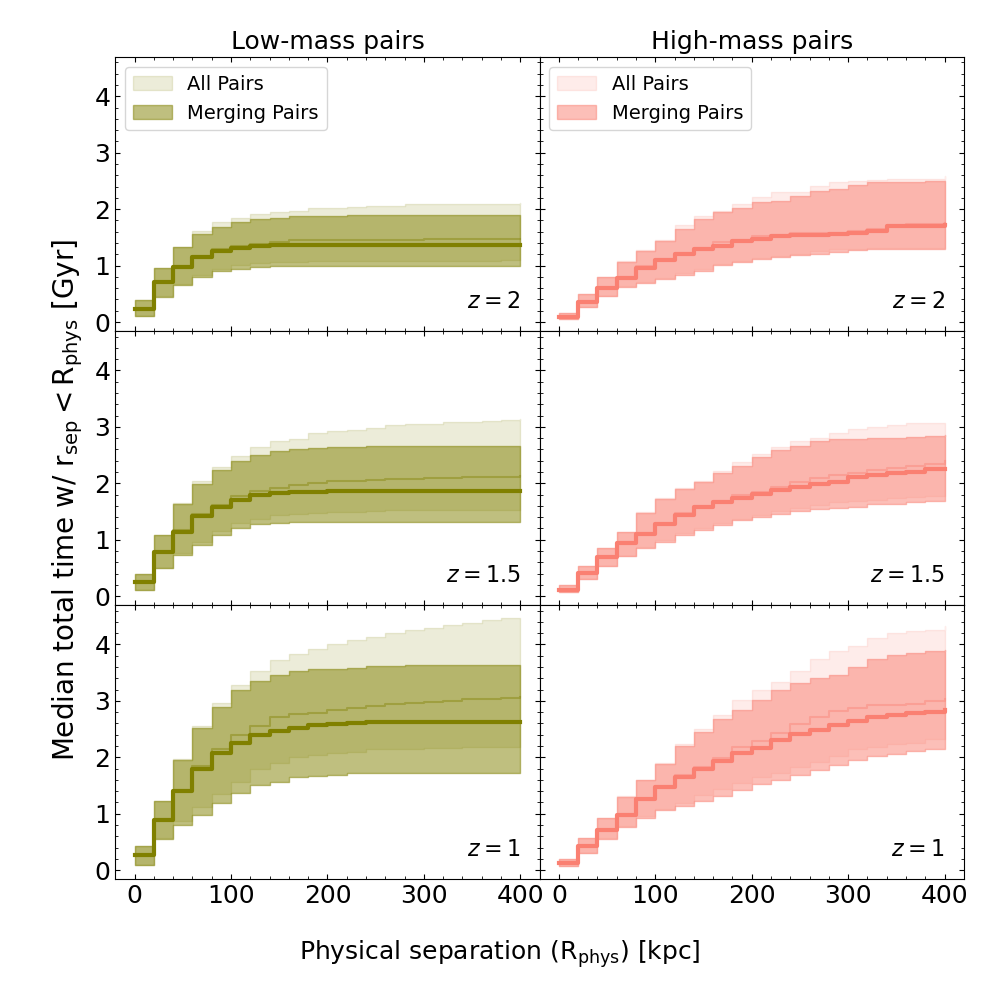
\includegraphics[width=\textwidth]{plots/bet-on-it/2_medtotal_LoHi.png}
%     \caption{\kc{reverse the direction of z} 
%     The median (solid) and 1st-3rd quartile spread (shaded regions) of the cumulative time that isolated low-mass pairs (left) and high-mass pairs (right) spend with separations \rsep{} between $10\kpc$ and \Rphys{}. 
%     The Merging Pairs sample (dark green and dark pink) selected at $z=(1,1.5,2)$ merge before $z=0$, while the All Pairs sample (light green and light pink) include all the pairs from the \paircat{} (mergers and non-mergers).  
%     The low-mass (high-mass) merging pairs represent XX\%(XX\%) of the low-mass (high-mass) pair sample at $z=1,1.5, \mbox{and } 2$ respectively. 
%     The sample of All Pairs spend more time at higher separations than the merging pairs, as expected since the non-merging pairs are not likely to have very low separations that would result in mergers prior to $z=0$. 
%     For a more direct comparison between the low-mass and high-mass pairs, see Fig.~\ref{fig:phys-vs-scaled}. 
%     }
%     \label{fig:low-vs-high}
% \end{figure*}

% \begin{figure*}[htb]
%     \centering
%     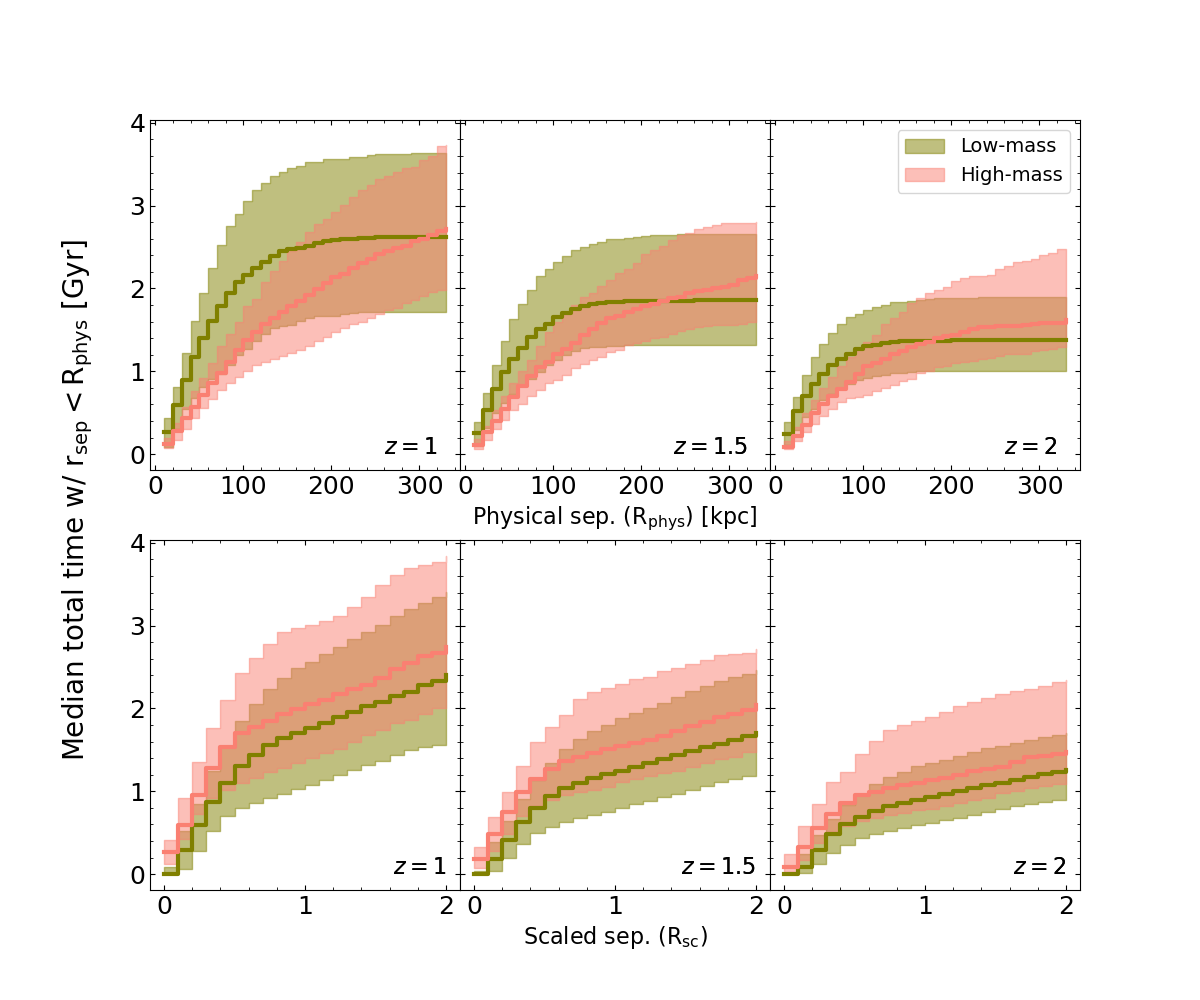
\includegraphics[width=\textwidth]{plots/bet-on-it/2_medtotal_PhScT.png}
%     \caption{\kc{Add legend to plot, and I think reverse the direction of z} 
%     The median and 1st-3rd quartile spread of the cumulative time that isolated merging pairs, selected at $z=(1,1.5,2)$, spend with separations \rsep{} greater than $10\kpc$ and less than either \Rphys{} or \Rsc{}.
%     %
%     (Top) The median total time spent by isolated merging pairs with separations between $10\kpc$ and \Rphys{}.
%     Low-mass pairs spend a longer amount of time within $\sim200\kpc$ than high-mass pairs at each of these redshifts. 
%     However, high-mass galaxies spend more time at higher separations of $\rsep>200-300\kpc$. This is because the elapsed time is measured starting at the infall snapshot of the pair, and high-mass halos have larger radii, the high-mass halo orbits have a broader distribution of separations that extend to larger separations than those of the low-mass pairs.
%     (Bottom) The median total time spent by pairs with separations greater than $\rsep>10\kpc$ and less than a given fraction of the virial radius ($\rsep/\Rvir<\Rsc$) of the pair, which scales with mass and redshift.  
%     High-mass pairs spend more time within the same scaled separation than low-mass pairs. For example, a high-mass pair selected from the $z=1.5$ sample will spend \kc{XXGyr} within \kc{$1\Rsc\sim XX\kpc$}, while a low-mass pair from the same sample will spend \kc{XXGyr} within \kc{$1\Rsc\sim XX\kpc$}. 
%     Low-mass and high-mass pairs have similar cumulative time profiles as a function of scaled separation, with a roughly constant offset for all scaled separations. 
%     The high-mass pairs spend a median of \kc{$XX\Gyr$} more than low-mass pairs at every scaled separation at $z=1$ and $z=1.5$, and a median of \kc{$XX\Gyr$} more $z=2$.
%     }
%     \label{fig:phys-vs-scaled}
% \end{figure*}



% ###########################################################################################
% Results II 
% ###########################################################################################



% \begin{figure*}[htb]
%     \centering
%     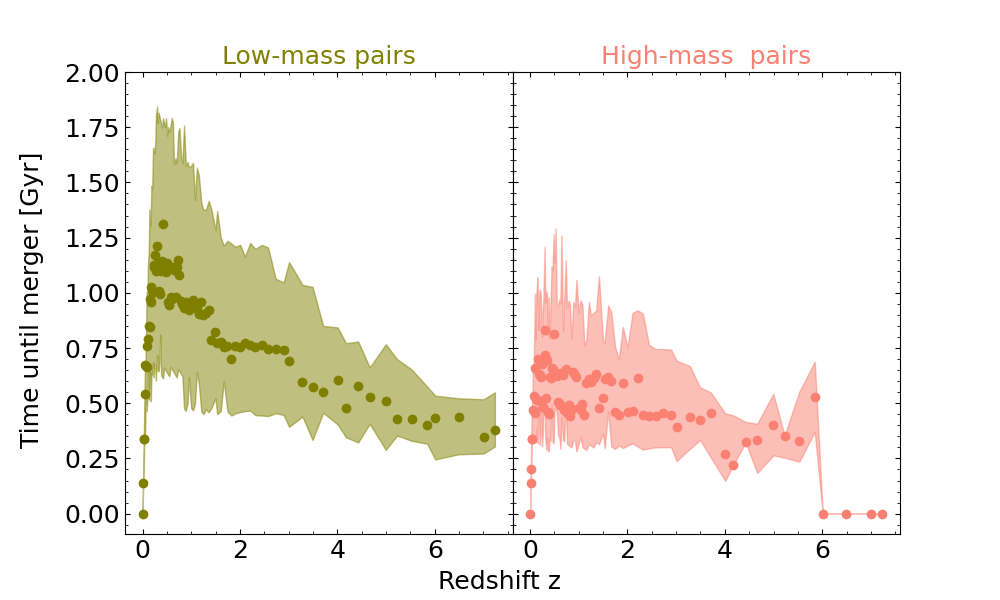
\includegraphics[width=\textwidth]{plots/bet-on-it/3_Timevsz.png}
%     \caption{}
%     % \label{fig:low-vs-high}
% \end{figure*}
% \begin{figure*}[htb]
%     \centering
%     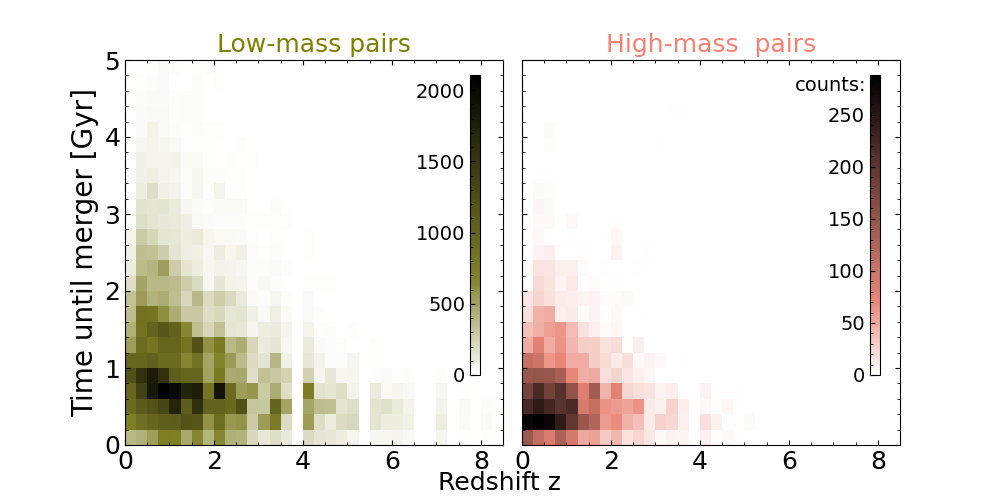
\includegraphics[width=\textwidth]{plots/bet-on-it/3_Timevsz-2d.png}
%     \caption{}
%     % \label{fig:low-vs-high}
% \end{figure*}
\begin{figure*}[htb]
    \centering
    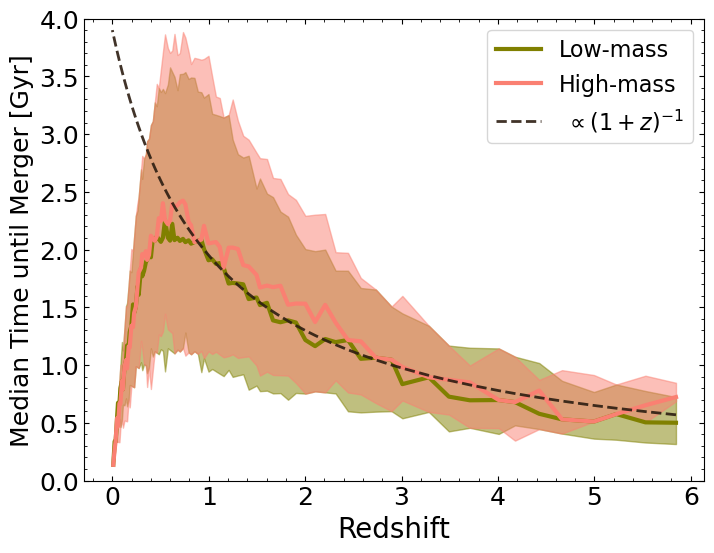
\includegraphics[width=\textwidth]{plots/bet-on-it/3_time_til_merger_full_fit.png}
    \caption{\kc{TODO: add LookbackTime vs. Z line, add Hubble time line} The median time until merger as a function of redshift for low-mass (green) and high-mass (pink) pairs. Shaded regions represent the 1st and 3rd quartile spread on the median. Pairs at each redshift are selected if they have experienced first infall. 
    % 
    The black dashed line shows the Hubble time, which bounds the median time until merger from $z=6$ to $z\sim0.5-0.75$.
    The dotted grey line shows the time to $z=0$ (the Lookback Time) as a function of redshift, which sets the upper bound for the time until merger that a merging pair can have. 
    The median time until merger is similar for low-mass and high-mass pairs, and rises from $z=6$ to a peak at $z\sim0.75$, then decreases to $z=0$.}
    \label{fig:timescales}
\end{figure*}

\begin{figure*}[htb]
    \centering
    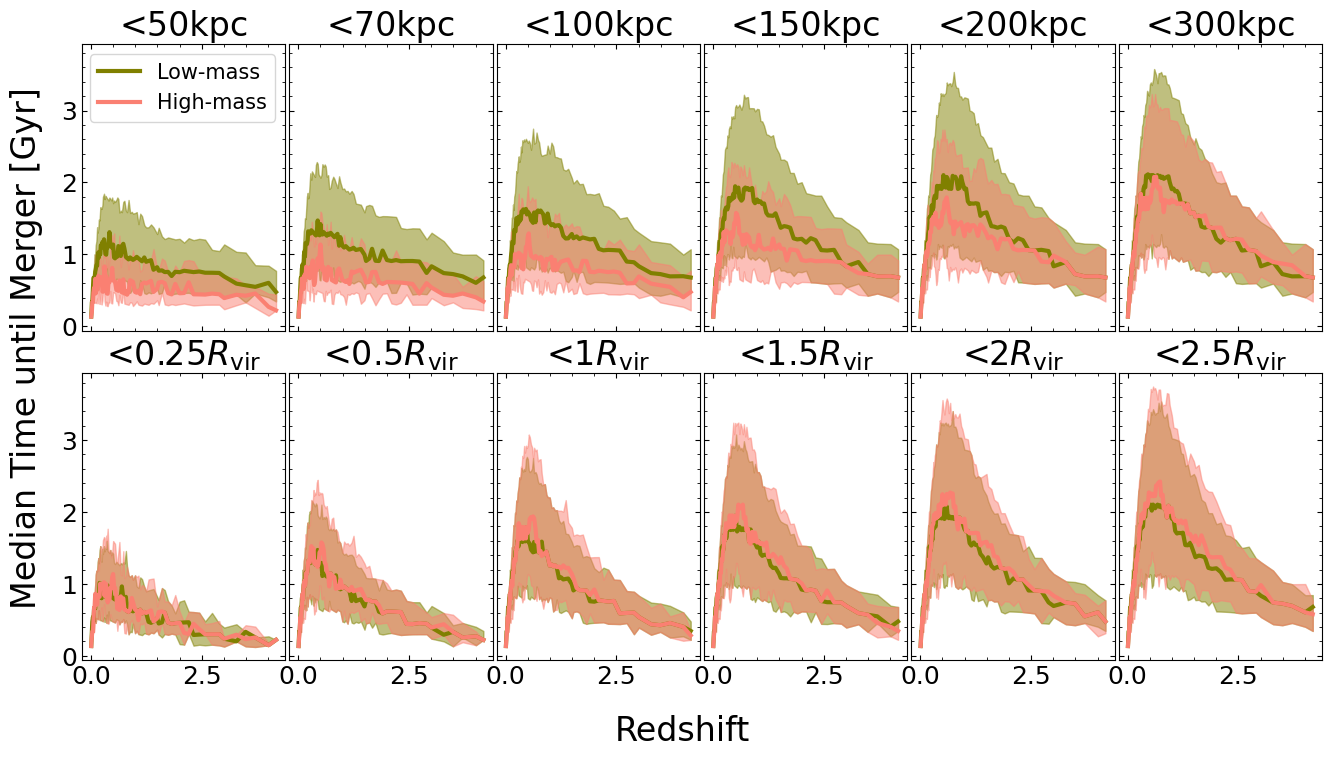
\includegraphics[width=\textwidth]{plots/bet-on-it/3_time_til_merger.png}
    \caption{(Top) The median time until merger as a function of redshift for low-mass (green) and high-mass (pink) pairs with 3D physical separations greater than $10\,\kpc$ and less than $(50,70,100,150,200,\mbox{and }300)\,\kpc$ from left to right. 
    (Bottom) The median time until merger as a function of redshift for pairs with physical separations greater than $10\,\kpc$ and less than $(0.25, 0.5, 1, 1.5, 2,\mbox{and }2.5)\,\Rvir$ from left to right. 
    % 
    The time until merger increases from $z=4$ to $z\sim0.5-0.75$, at which point the time until merger decreases to zero since all low redshift mergers must have short merger timescales to merge before the end of the simulation at $z=0$. 
    }
    \label{fig:timescales-sep}
\end{figure*}


\section{Discussion}
% \subsection{Merger Rates for Dwarf Pairs}
% % - What combination of values best reproduces the merger fraction acquired from the sims?
% % Do you need the scale of merger probability as in Ventou to get the match?
% % Vicente & Casteels 2014 comparison (pair fractions plot)
% \subsection{Pairs of Dwarfs That Do Not Merge}
% % can talk about the unmerged fraction merger rates here
% \subsection{Choosing Samples at Lower and Higher Redshift}
% % can also compare to samples to merger fractions and merger rates chosen at z=1 and z=2 (plots you have already)
% \subsection{Comparing with Merger Rates for Massive Galaxy Pairs}
% % compare to massive pairs in both obs window and merger rate
% % compare back to the assumption of isolation


\section{Summary and Conclusions}

% To do:
% -Sample: starting with FoF group cut and always show the total sample (merged and unmerged) since the unmerged sample is so small
% -Keep Fig 1: (two panels) add in a few more orbits to show the diversity and then have a panel to show one example where you shade everything below 100 kpc to show how the total time at S is computed
% -Keep Figure 2 as is 
% -Remove Figure 3
% -Figure 4: remove normalization of both samples so it's clear that the unmerged ones spend a lot of time at high separation and that they are a small percent of the fraction (put this in discussion or an appendix)
% -Remove Fig 5 and state conclusions in words along with the FoF group selection (most pairs have been in the same group for 1.5 Gyr) (can quote percentages from a cumulative version of the plot, or sum)
% -Figure 6: only show the *full* sample with the FoF group cut 
% check the half mass radius of the most massive dwarfs in your sample and justify 10 kpc by saying you want to be able to resolve twice that 









% \section{Discussion}

** 
\appendix
\begin{figure*}[htb]
    \centering
    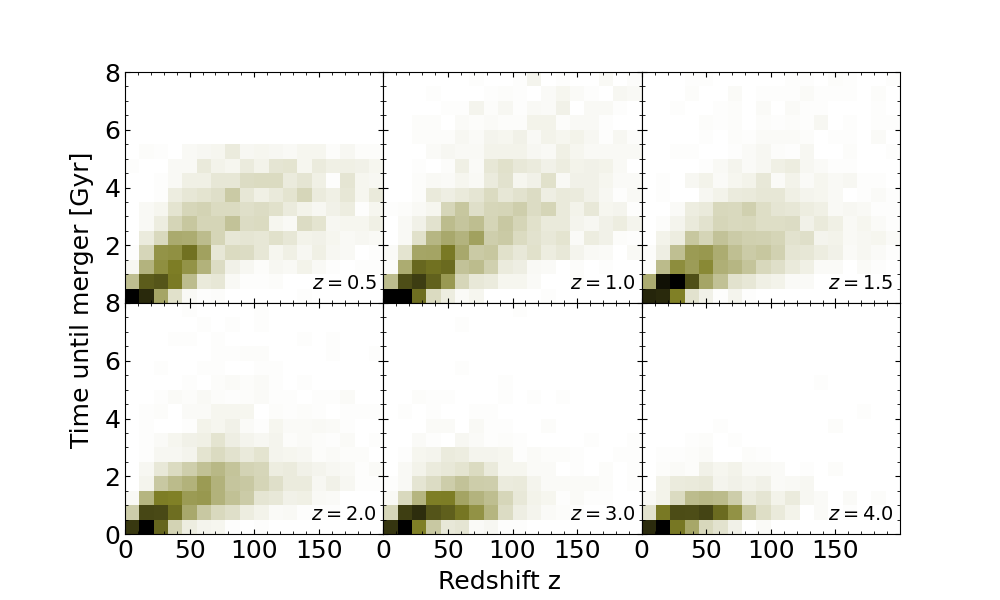
\includegraphics[width=\textwidth]{plots/bet-on-it/3_Timevsseplow-2d.png}
    \caption{}
    % \label{fig:low-vs-high}
\end{figure*}

\begin{figure*}[htb]
    \centering
    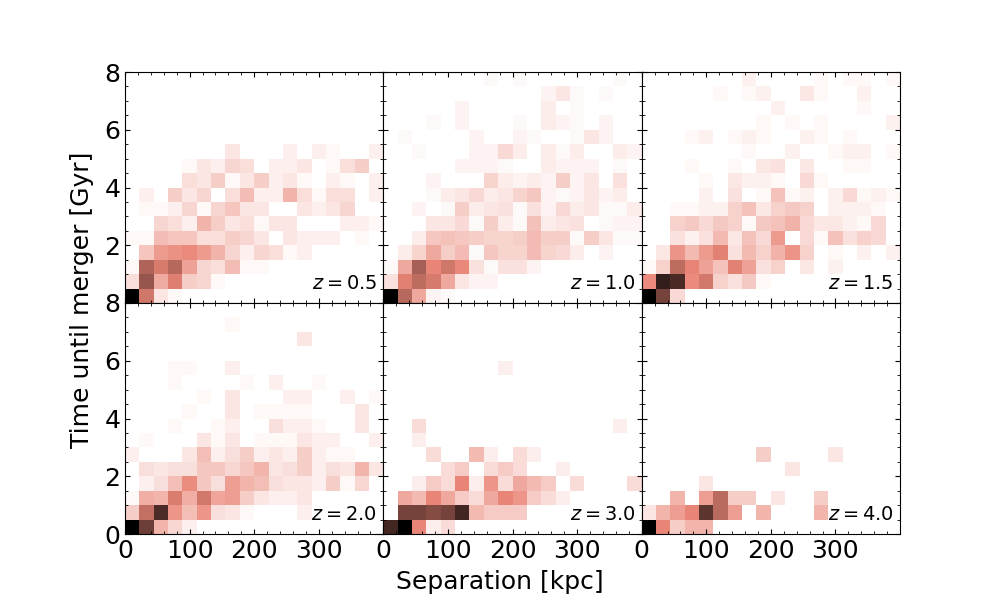
\includegraphics[width=\textwidth]{plots/bet-on-it/3_Timevssephigh-2d.png}
    \caption{}
    % \label{fig:low-vs-high}
\end{figure*}
% \begin{figure}[htb]
%     \centering
%     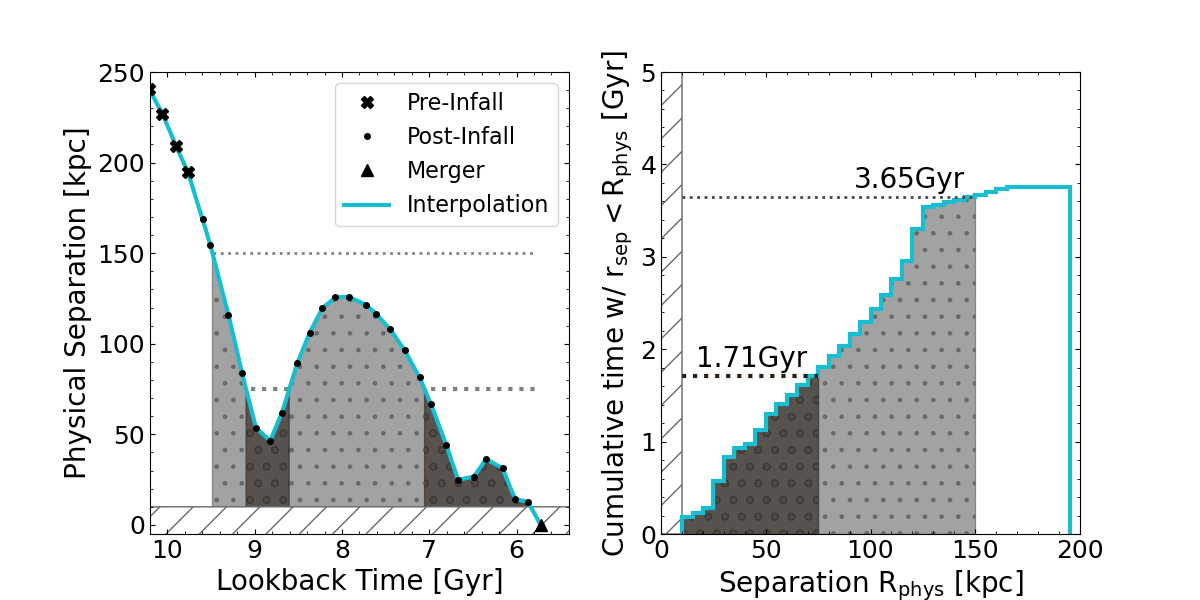
\includegraphics[width=0.5\columnwidth]{plots/bet-on-it/4_example1.png}
% \end{figure}
% \begin{figure}[htb]
%     \centering
%     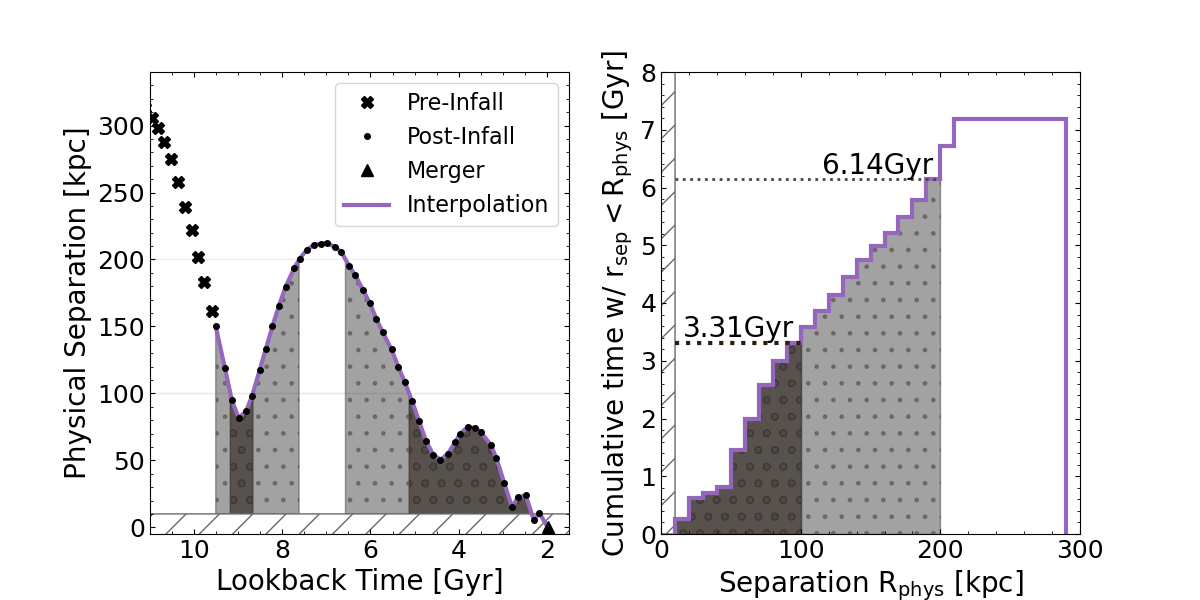
\includegraphics[width=0.5\columnwidth]{plots/bet-on-it/4_example2.png}
%     \caption{}
% \end{figure}
% \begin{figure}[htb]
%     \centering
%     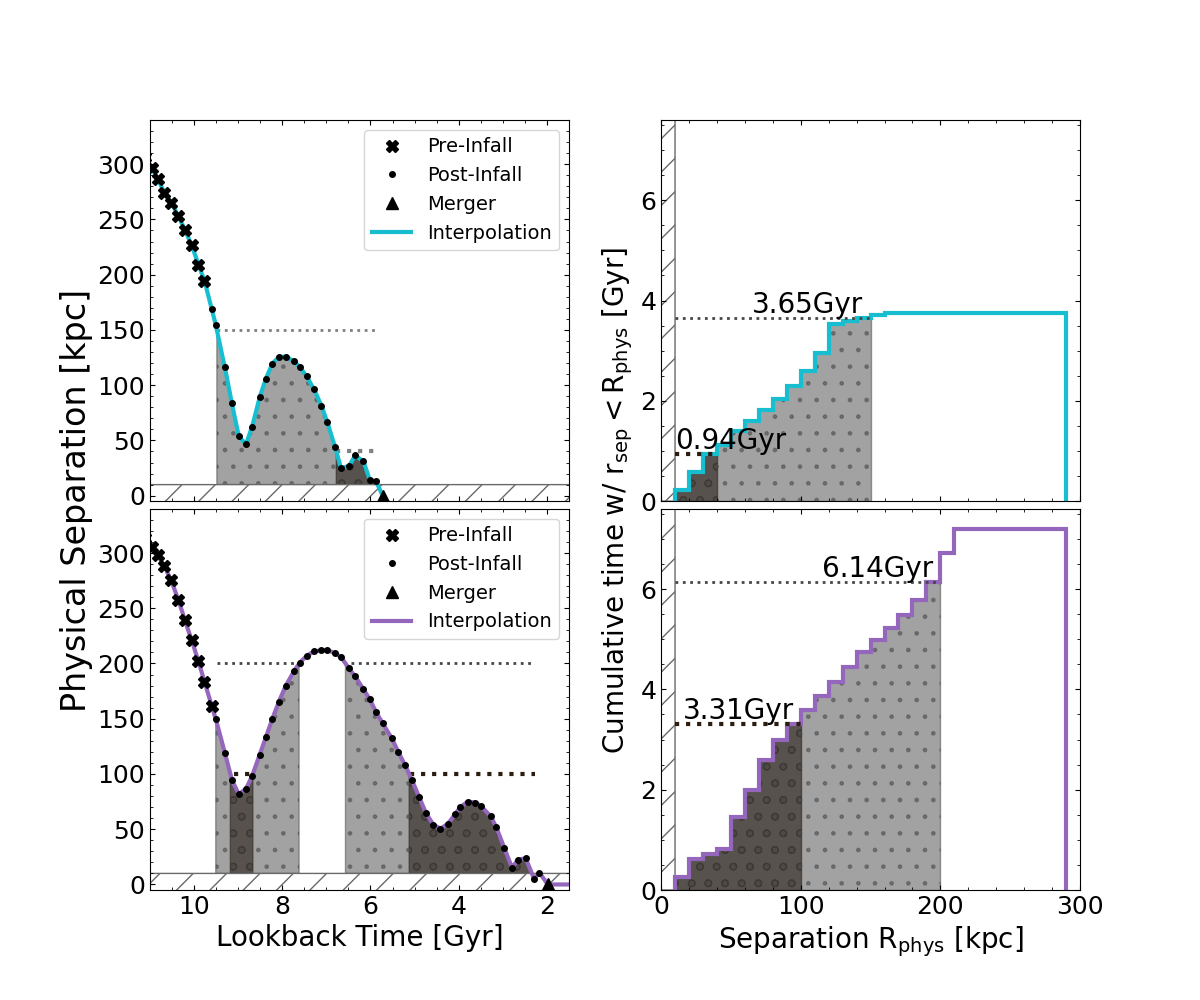
\includegraphics[width=0.5\columnwidth]{plots/bet-on-it/4_examplecombo.png}
% \end{figure}

% \begin{figure}[htb]
%     \centering
%     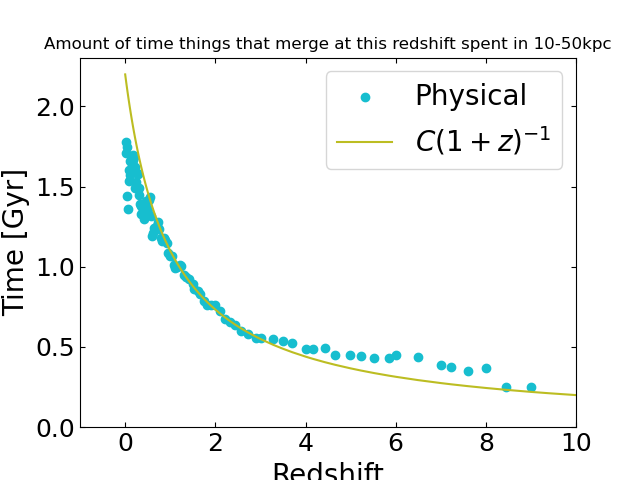
\includegraphics[width=0.5\columnwidth]{plots/bet-on-it/3_timeinbin_beforemerger.png}
% \end{figure}
% \begin{figure}[htb]
%     \centering
%     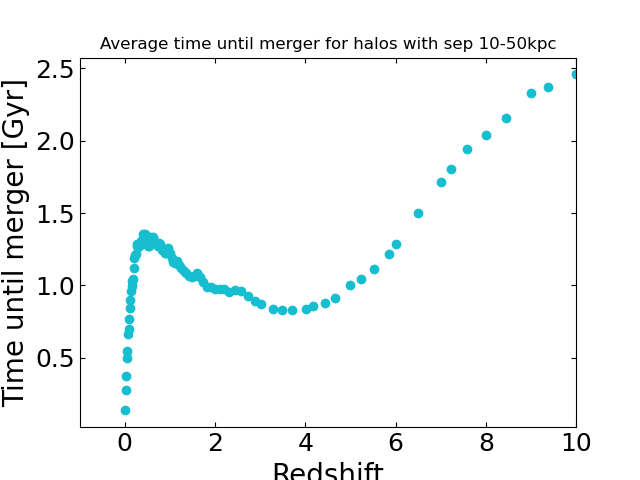
\includegraphics[width=0.5\columnwidth]{plots/bet-on-it/3_timeinbin_untilmerger_phys.png}
% \end{figure}

% \begin{figure*}[htb]
%     \centering
%     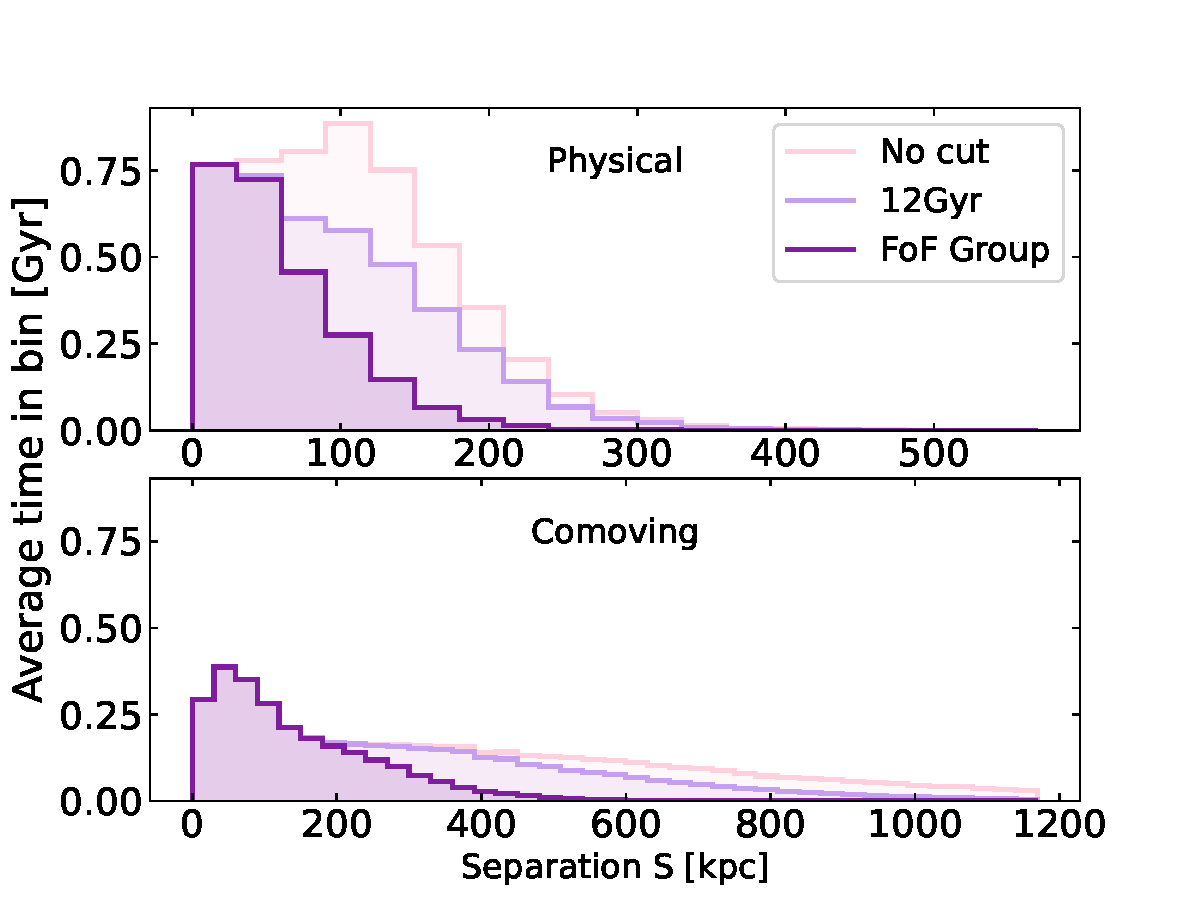
\includegraphics[width=\columnwidth]{plots/4_timescales/timevssep_phys+co.pdf}
%     \caption{}
%     % \label{fig:phys-comoving}
% \end{figure*}

% \begin{figure*}[htb]
%     \centering
%     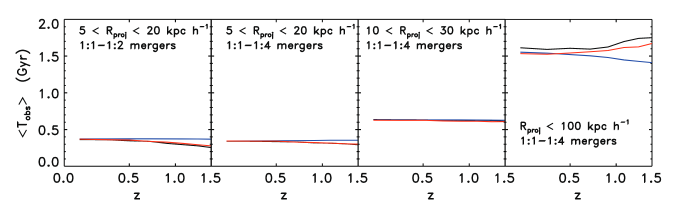
\includegraphics[width=\columnwidth]{lotz.png}
%     \caption{}
%     % \label{fig:phys-comoving}
% \end{figure*}







\bibliography{refs}{}
\bibliographystyle{aasjournal}

\end{document}

